% ============================================================================
% Merged oral presentation — IM06 project / MedVAE
% Order of the parts: 1) Elias  2) Théophile  3) Yanic  4) Théo
% All figures are in figures/<firstname>/...
% ============================================================================
\documentclass[aspectratio=169]{beamer}

% ---------- Packages ----------
\usepackage[utf8]{inputenc}
\usepackage[T1]{fontenc}
\usepackage[english]{babel}
\usepackage{graphicx}
\usepackage{amsmath,amssymb}
\usepackage{hyperref}
\usepackage{pifont}
\usepackage{booktabs}
\usepackage{xcolor}
\usepackage{colortbl}

\newcommand{\cmark}{\textcolor{green!50!black}{\ding{51}}}
\newcommand{\xmark}{\textcolor{red!70!black}{\ding{55}}}
\DeclareMathOperator*{\argmin}{arg\,min}

% Look for figures in all subfolders
\graphicspath{%
  {figures/}%
  {figures/elias/}{figures/theophile/}{figures/yanic/}{figures/theo/}%
}

% ---------- Theme ----------
\usetheme{Madrid}
\usecolortheme{default}

\definecolor{TPBordeaux}{RGB}{140,30,45}
\setbeamercolor{structure}{fg=TPBordeaux}

% Automatic section page
\AtBeginSection[]{%
  \begin{frame}[plain,c]
    \begin{center}
      \usebeamercolor[fg]{structure}%
      {\Large\bfseries\insertsection}
    \end{center}
  \end{frame}%
}

% ---------- Title info ----------
\title[MedVAE — Coronary segmentation]{MedVAE: adaptation, fine-tuning and analysis for medical imaging and coronary segmentation}
\author{Yanic Rothlingshofer  \and Théo Palagi \and Elias Corlou \and Théophile Nadiedjoa}
\institute[]{\large \it Télécom Paris}
\date{\underline{Supervisor:} Elsa Angelini}

% ---------- Logo (shown if logo_TP.png is next to the .tex) ----------
\titlegraphic{%
  \vspace{0cm}
  
\includegraphics[width=0.3\linewidth]{logoTP.png}%
  }%


\begin{document}

\maketitle

% ############################################################################
% INTRODUCTION (from final.tex, Sec. Introduction)
% ############################################################################
\begin{frame}{Introduction}
  \begin{columns}[T]
  \begin{column}{0.58\textwidth}
  \textbf{Context.} Deep learning in medical imaging is limited by the high
  resolution required for diagnostic detail. VAEs compress the image into a
  compact latent.
  \begin{itemize}
    \item \textbf{MedVAE}: generic medical compressor ($>1$M images),
      $\times 4$ per side, $\times 16$ in area ($512^2 \to 128^2 \times 1$), trained in two stages
      (reconstruction then semantic enrichment).
  \end{itemize}
  \vspace{0.4em}
  \textbf{Domain.} Coronary angiography (ARCADE, $1\,500$ images):
  thin, tubular, low-contrast structures, noise and artifacts.
  \end{column}
  \begin{column}{0.42\textwidth}
  \begin{block}{Central question}
  Does a generic medical compressor remain \alert{reliable and useful} when
  facing a specific and demanding clinical domain?
  \end{block}
  \vspace{0.2em}
  \footnotesize \textbf{Four complementary axes:}
  \begin{enumerate}
    \item Robustness to degradations
    \item Image-quality inductive bias via FiLM
    \item Semantic structuring of the latent (JEPA)
    \item Latent representation for segmentation
  \end{enumerate}
  \end{column}
  \end{columns}
\end{frame}

% ############################################################################
% PART 1 — ELIAS
% Figures available in figures/elias/ :
%   degradation_visual.png, pipeline_corrected.pdf, mpsnr.pdf, robustness_corrected.png,
%   179_clean.png, 179_clean_ov.png, 179_deg_ov.png, 179_poisson.png,
%   metrics_by_level_all_masked.pdf,
%   metrics_by_level_masked_blur_NEW.png,
%   metrics_by_level_masked_jpeg_NEW.png,
%   metrics_by_level_masked_poisson_NEW.png
% ############################################################################
\section{Robustness of MedVAE to input degradations}

\begin{frame}{Method: evaluation protocol}
\centering
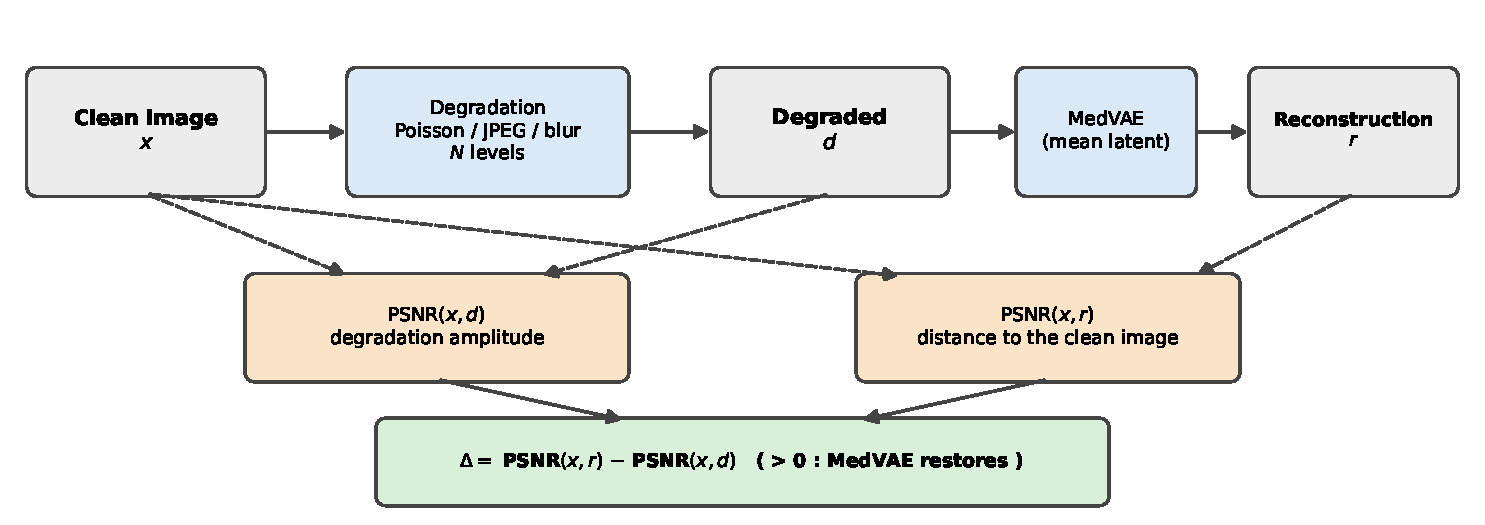
\includegraphics[width=0.85\linewidth]{elias/pipeline_corrected.pdf}

\vspace{0.6em}
\footnotesize The reconstruction is compared to the \alert{clean} image: does MedVAE bring a degraded input closer to it?
100 \texttt{seg\_val} images, deterministic latent, fixed intensity scale, seeded noise, bootstrap CIs.
\end{frame}

\begin{frame}{Why not a no-reference metric?}
\begin{columns}[T]
\begin{column}{0.56\textwidth}
\small
Discarded approach: score the input quality with ARNIQA (no-reference), then correlate it with the reconstruction quality.

\vspace{1.5em}
\centering
\footnotesize
\begin{tabular}{@{}ll@{}}
\toprule
\multicolumn{2}{l}{\textbf{ARNIQA — clean dataset (n=1000)}} \\
\midrule
min / max & 0.2695 / 0.6512 \\
mean $\pm$ std & 0.4570 $\pm$ 0.0482 \\
quantiles 5/50/95 & 0.3772 / 0.4566 / 0.5391 \\
\bottomrule
\end{tabular}

\vspace{1.4em}
\raggedright
\alert{Significant but weak correlation}: the intrinsic quality variance between clean images is too small to serve as an exploitable axis.
\end{column}
\begin{column}{0.44\textwidth}
\centering
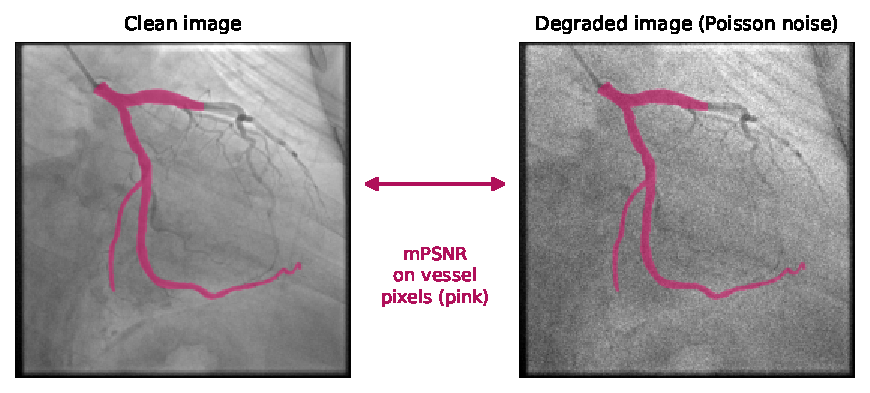
\includegraphics[width=0.68\textwidth]{elias/mpsnr.pdf}

\vspace{0.3em}
\tiny mPSNR illustration (vessel mask)
\end{column}
\end{columns}
\end{frame}

\begin{frame}{Result: MedVAE removes noise, not blur or JPEG artefacts}
\begin{columns}[T]
\begin{column}{0.46\textwidth}
\centering
\footnotesize
\vspace{0.3em}
\begin{tabular}{@{}lcc@{}}
\toprule
Degradation & $\Delta$ PSNR (dB) & Restored \\
\midrule
Poisson & $+1.2 \to +6.6$ & $99$--$100\%$ \\
JPEG ($95 \to 5$) & $-11.7 \to -0.6$ & $0$--$9\%$ \\
Blur & $-2.0 \to +0.1$ & -- \\
\bottomrule
\end{tabular}

\vspace{0.3em}
\tiny $\Delta = \mathrm{PSNR}(\text{clean}, \text{recon}) - \mathrm{PSNR}(\text{clean}, \text{degraded})$
\end{column}
\begin{column}{0.54\textwidth}
\footnotesize
\begin{itemize}
  \item \textbf{Poisson}: genuine denoising, larger for stronger noise
  \item \textbf{JPEG}: never restored --- MedVAE's own error (33 dB ceiling) exceeds the artefacts
  \item \textbf{Blur}: not restored --- the reconstruction follows the blurred input
  \item \alert{The earlier ``blur reconstructs better''} measured fidelity to the \emph{degraded} input (orange)
\end{itemize}
\end{column}
\end{columns}
\end{frame}

\begin{frame}{Result: restoration curves (vessel pixels)}
\centering
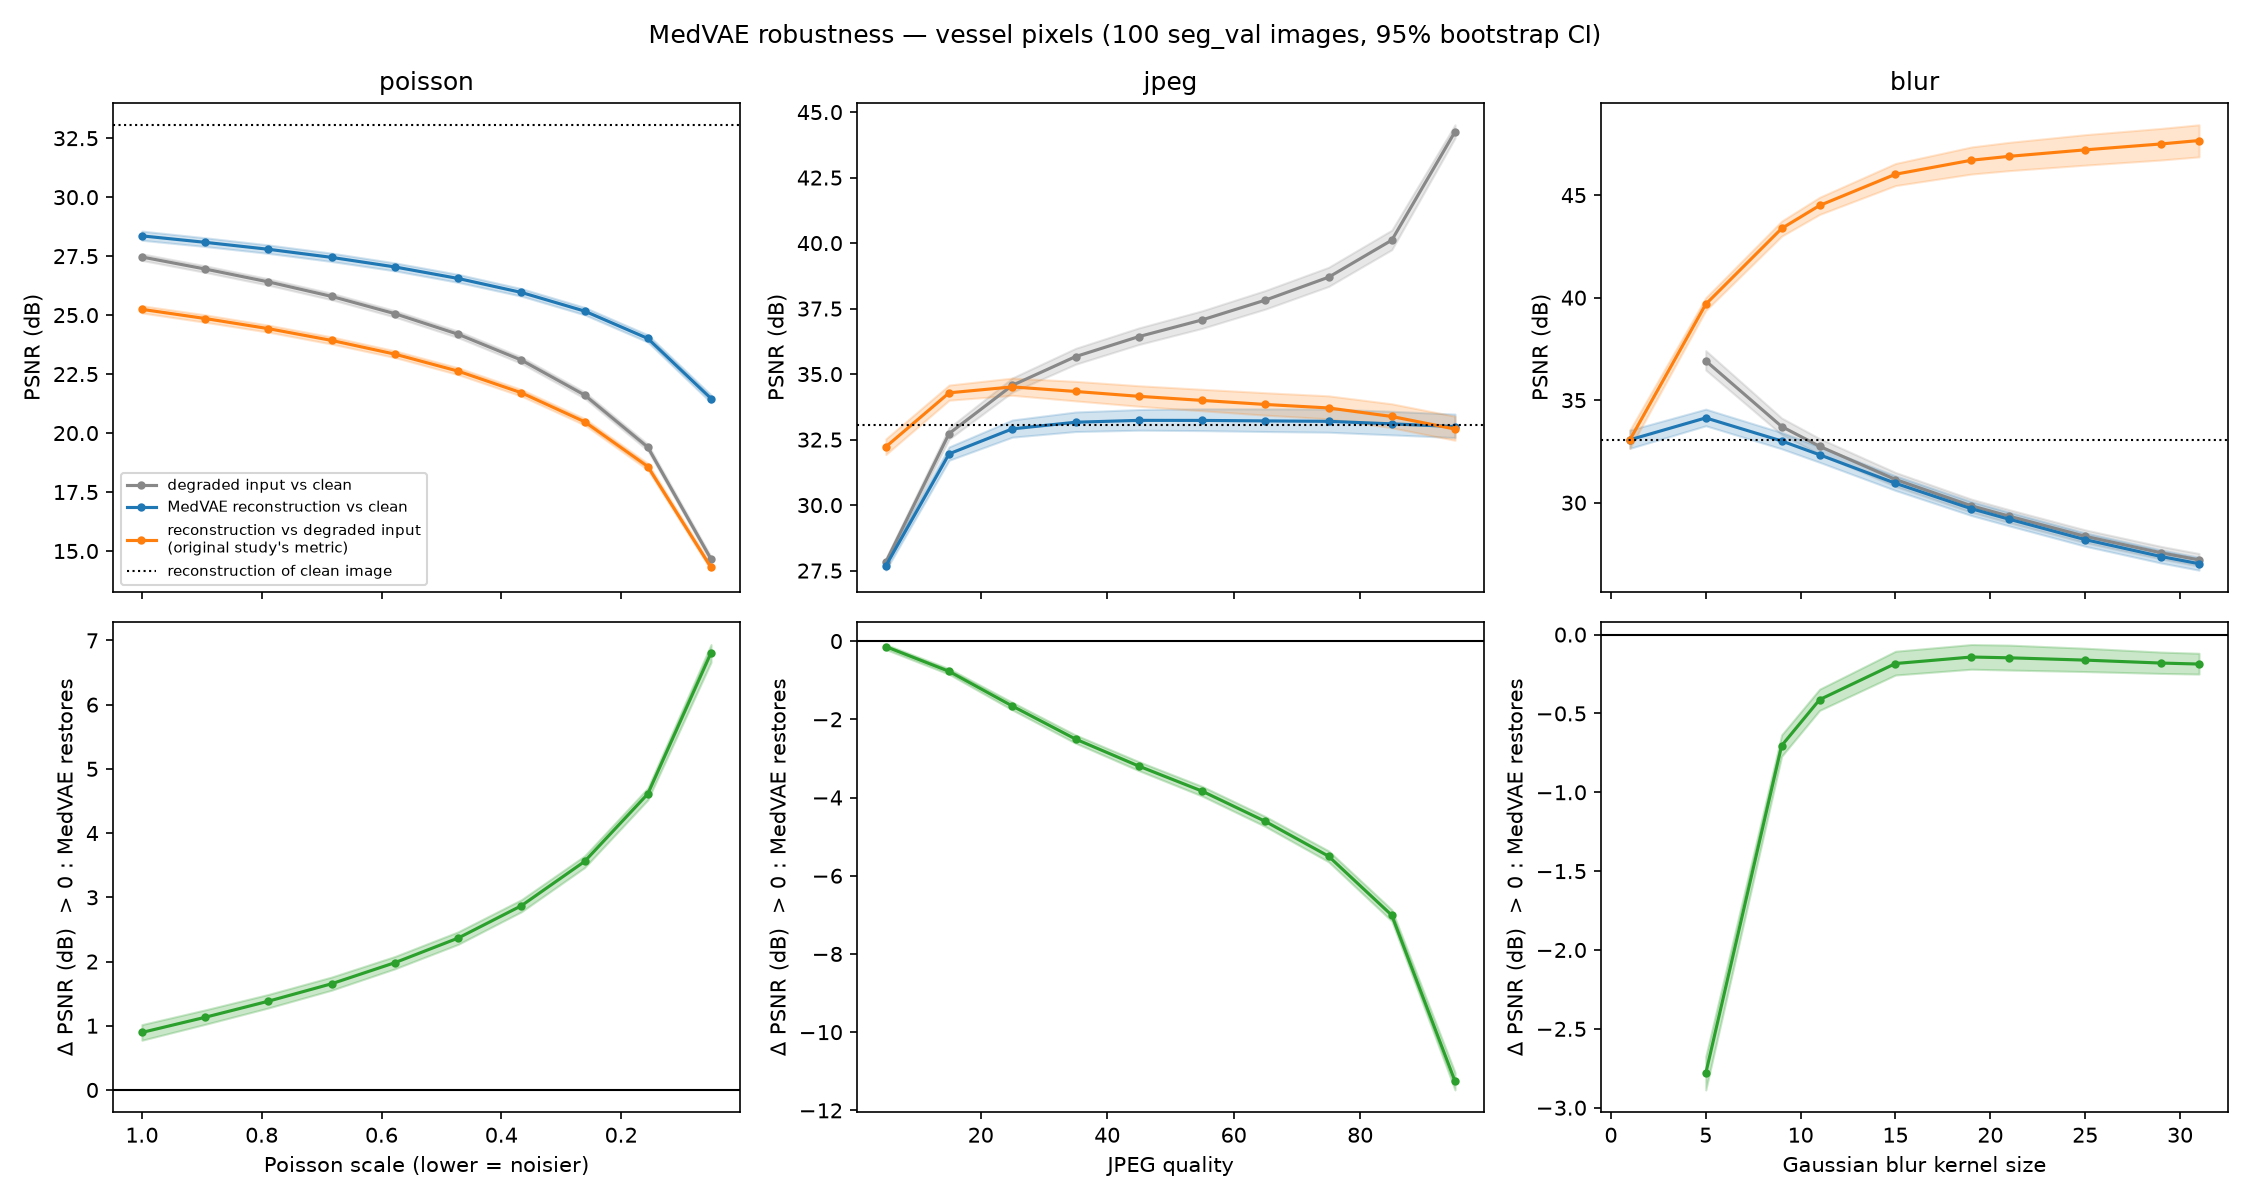
\includegraphics[height=0.74\textheight]{elias/robustness_corrected.png}

\footnotesize Grey: degraded input vs clean. Blue: reconstruction vs clean. Orange: reconstruction vs degraded input (earlier metric). Bottom: $\Delta$.
\end{frame}

% ############################################################################
% PART 2 — THÉOPHILE
% Image-quality inductive bias for MedVAE (conditioning via FiLM)
% Figures in figures/theophile/
% ############################################################################
\section{Image-quality inductive bias (FiLM)}

% Motivation
\begin{frame}{Motivation}
  \begin{itemize}
    \item MedVAE applies the \textbf{same transform} to a clean or a heavily
      degraded coronary angiography: no notion of \emph{how degraded} the
      input is.
    \item \textbf{Hypothesis:} conditioning MedVAE on a quality score
      $c \in [0,1]$, injected via FiLM, should let it adapt to the
      degradation level actually present.
    \item Three independent ways to compute $c$ (A: weighted, B: PCA,
      C: learned): in-depth study with C (3 seeds), checks with A and B.
  \end{itemize}
\end{frame}

% Quality score construction
\begin{frame}{Building the quality score $c$}
  \begin{center}
    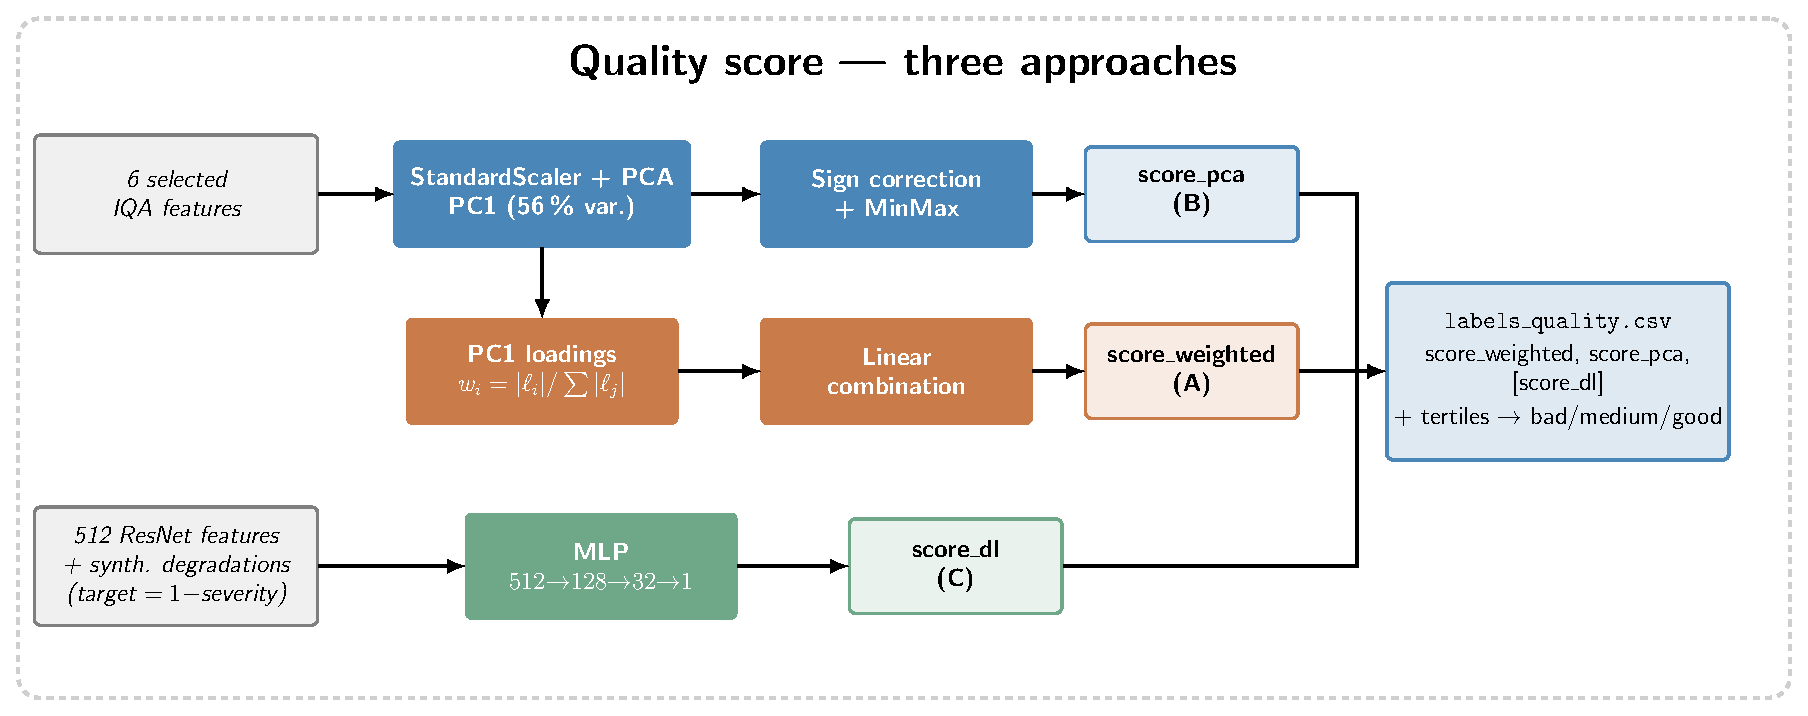
\includegraphics[width=0.95\textwidth]{theophile/pipeline_B_score.pdf}
  \end{center}
\end{frame}

% Sanity check on the score
\begin{frame}{Does the score make clinical sense?}
  \begin{center}
    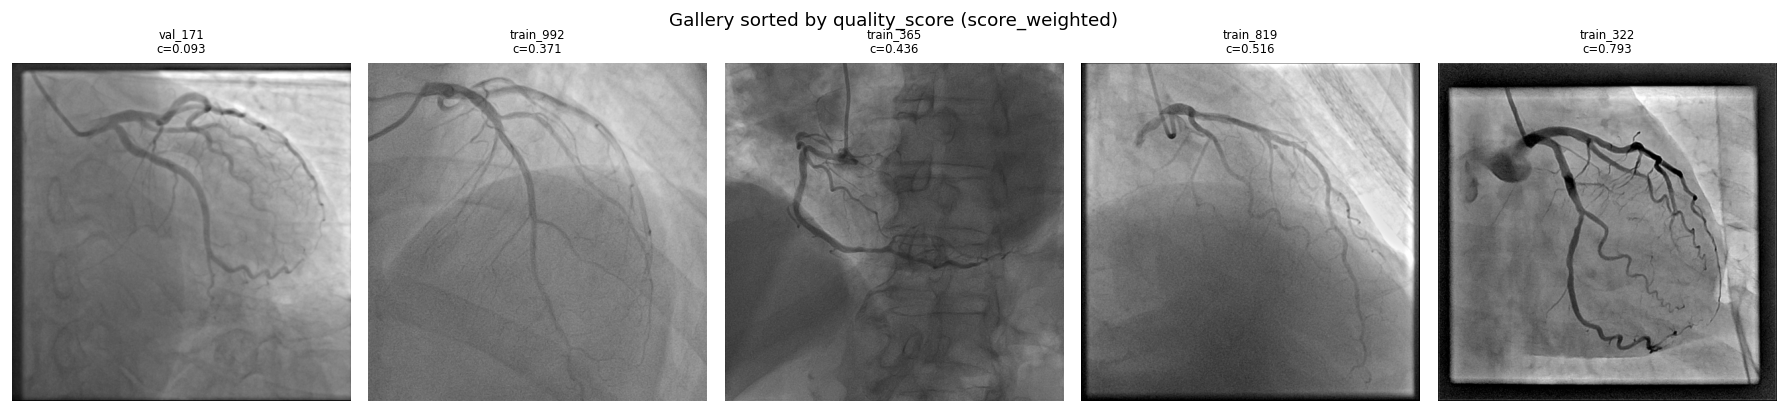
\includegraphics[width=\textwidth]{theophile/result_gallery_score.png}
  \end{center}
  \begin{center}
    \footnotesize ARCADE images sorted by increasing score $c$ (approach A).
  \end{center}
\end{frame}

% FiLM conditioning + revised protocol
\begin{frame}{FiLM conditioning \& revised protocol}
  \begin{center}
    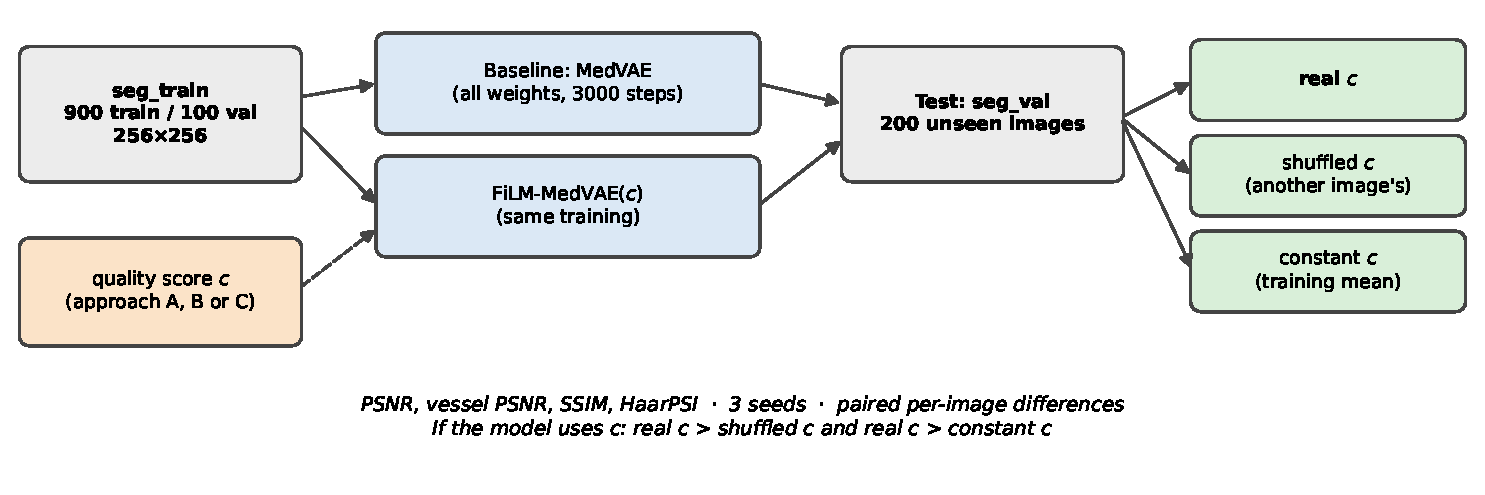
\includegraphics[width=0.92\textwidth]{theophile/pipeline_film_corrected.pdf}
  \end{center}
  \footnotesize
  \begin{itemize}
    \item FiLM after each of the 19 ResNet blocks: $h \leftarrow (1+\gamma(c))\,h + \beta(c)$, zero-initialised (+1.7M parameters, +3\,\%)
    \item \alert{Revised}: $256\times256$ (was $64\times64$, where MedVAE only reaches 20.7 dB), KL normalised per pixel, same training for both models, 3 seeds
  \end{itemize}
\end{frame}

% Main result
\begin{frame}{Result: fine-tuning helps, conditioning does not}
  \begin{center}
    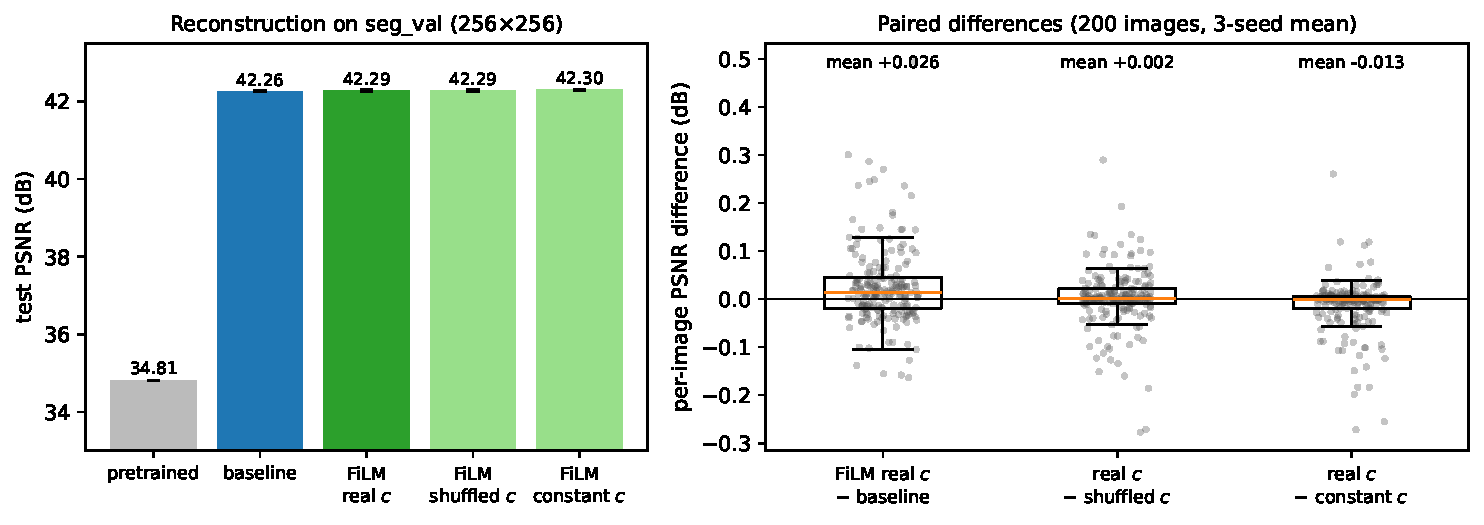
\includegraphics[width=\textwidth]{theophile/film_results.pdf}
  \end{center}
  \footnotesize
  \begin{itemize}
    \item Fine-tuning MedVAE on ARCADE: \textbf{+7.4 dB} (vessels: +5.3 dB), same for all seeds
    \item FiLM vs baseline: +0.03 dB --- negligible
  \end{itemize}
\end{frame}

% Is c used?
\begin{frame}{Does the network use $c$?}
  \begin{columns}[T]
  \begin{column}{0.5\textwidth}
  \centering\footnotesize
  \begin{tabular}{@{}lc@{}}
  \toprule
  Paired difference (PSNR) & dB \\
  \midrule
  true $c$ $-$ shuffled $c$ & $+0.002$ \\
  true $c$ $-$ constant $c$ & $-0.013$ \\
  \midrule
  \multicolumn{2}{@{}l}{\emph{Checks (seed 42)}} \\
  Score C, FiLM lr $\times100$: true $-$ constant & $-0.001$ \\
  Score A: true $-$ shuffled & $+0.009$ \\
  Score B: true $-$ shuffled & $+0.037$ \\
  \bottomrule
  \end{tabular}
  \end{column}
  \begin{column}{0.5\textwidth}
  \footnotesize
  \begin{itemize}
    \item \textbf{Score C: no}. Another image's score, or a constant, does as well
    \item \textbf{Scores A, B: barely} ($\leq 0.04$ dB)
    \item FiLM gains come from the added parameters, not from the quality information
    \item $c$ is computed \emph{from the image}: for an autoencoder of that image, it carries nothing new
    \item \alert{The earlier ``only C is exploited''} compared two separately trained single runs
  \end{itemize}
  \end{column}
  \end{columns}
\end{frame}

% ############################################################################
% PART 3 — YANIC
% Semantic structuring of the latent space (JEPA vs BioMedCLIP)
% Figures in figures/yanic/
% ############################################################################
\section{Semantic structuring of the latent space (JEPA)}

\begin{frame}{Original stage 2 — BioMedCLIP distillation}
  \centering
  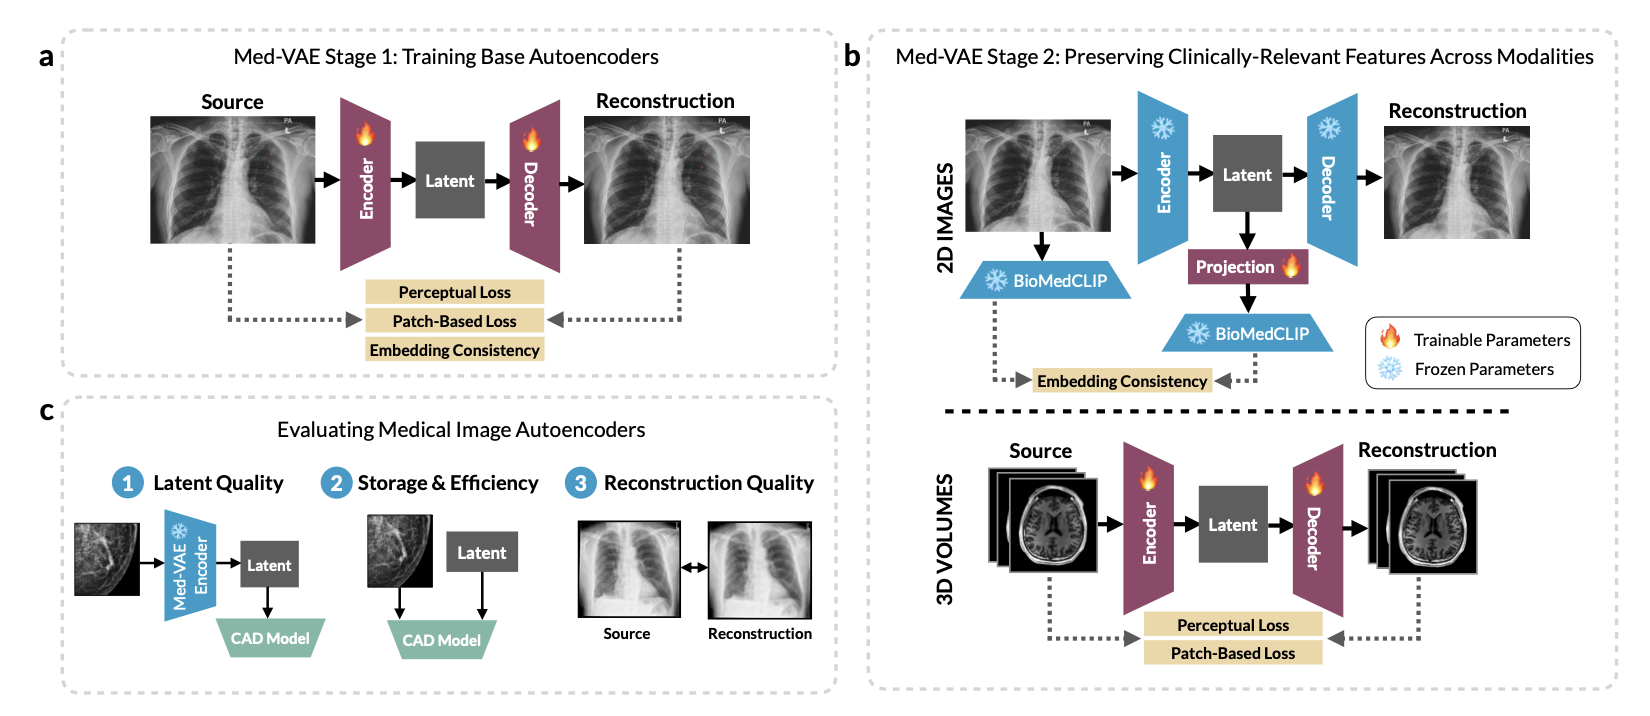
\includegraphics[width=1.0\linewidth]{yanic/pipeline_ori.png}
\end{frame}

\begin{frame}{Modified stage 2 — JEPA adaptation}
  \centering
  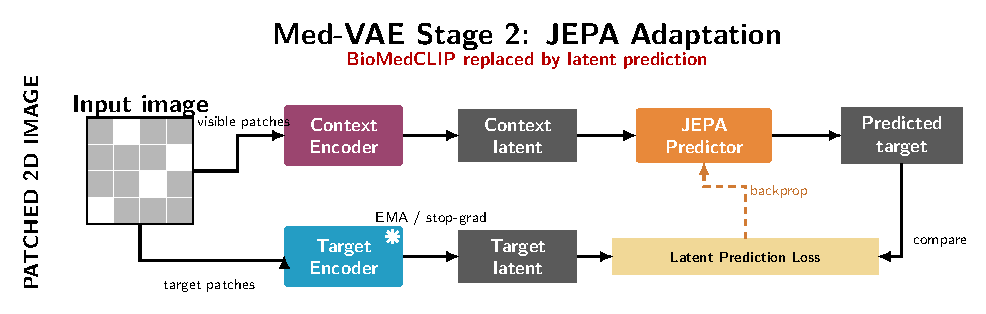
\includegraphics[width=0.72\linewidth]{yanic/stage_2_pipeline.pdf}

  \vfill
  {\small
  \[\boxed{
    \mathcal{L}_{\text{stage2}}
    = \mathcal{L}_{\text{pred}}
    + \lambda_{\text{SIGReg}}\,\mathcal{L}_{\text{SIGReg}}
  }\]
  \[
    \mathcal{L}_{\text{pred}}
    = \frac{1}{|\mathcal{M}|} \sum_{p \in \mathcal{M}}
      \mathrm{SmoothL_1}\!\left(\hat{z}_t^{(p)},\, \tilde{z}_t^{(p)}\right),
    \qquad
    \mathcal{L}_{\text{SIGReg}}
    = \mathbb{E}_{\mathbf{v}}\!\left[ T_{\text{EP}}\!\left(\bigl\{ z_c^\top \mathbf{v} \bigr\}\right) \right]
  \]}
\end{frame}

\begin{frame}{Revised evaluation}
  \small
  \begin{itemize}
    \item \textbf{Stage 1 is not MedVAE}: same family, but smaller (21M), $\times8$ per side, trained \emph{from scratch} on ARCADE
    \item \alert{Earlier issues}: test images in the pre-training; the ``25 dimensions for 90\,\% of the variance'' measured \texttt{channel\_proj}, a layer \emph{never trained}
    \item Now: retrained without the test set; evaluated on the layer JEPA trains (features before \texttt{conv\_out}), 300 test images
  \end{itemize}
  \vspace{0.3em}
  \centering\footnotesize
  \begin{tabular}{@{}lccc@{}}
  \toprule
   & MedVAE & Stage 1 & Stage 2 JEPA \\
  \midrule
  PSNR (dB) & 34.8 & 30.2 & 17.8 \\
  Vessel linear probe (Dice) & 0.517 & \textbf{0.541} & 0.485 \\
  Effective rank / dims for 90\,\% var. & 251 / 61 & 111 / 22 & 139 / 34 \\
  \bottomrule
  \end{tabular}
\end{frame}

\begin{frame}{Results — reconstruction and features}
  \centering
  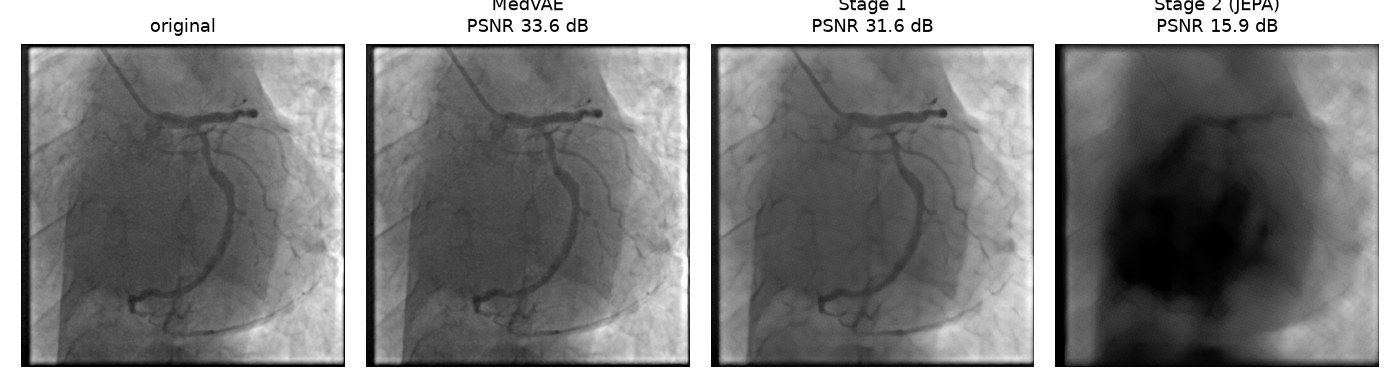
\includegraphics[width=0.8\linewidth]{yanic/recon.png}

  \vspace{0.2em}
  {\footnotesize
  \begin{itemize}
    \item \alert{Frozen} decoder: the adapted encoder is no longer decodable (17.8 dB)
    \item JEPA \textbf{degrades} vessel separability ($-0.056$ vs stage 1), \textbf{no contraction} (rank $111 \to 139$, as SIGReg intends)
    \item Learning on angiographies helps (stage 1 $>$ MedVAE), JEPA does not
  \end{itemize}}
\end{frame}

\begin{frame}{Results — RGB PCA of the intermediate features}
  \centering
  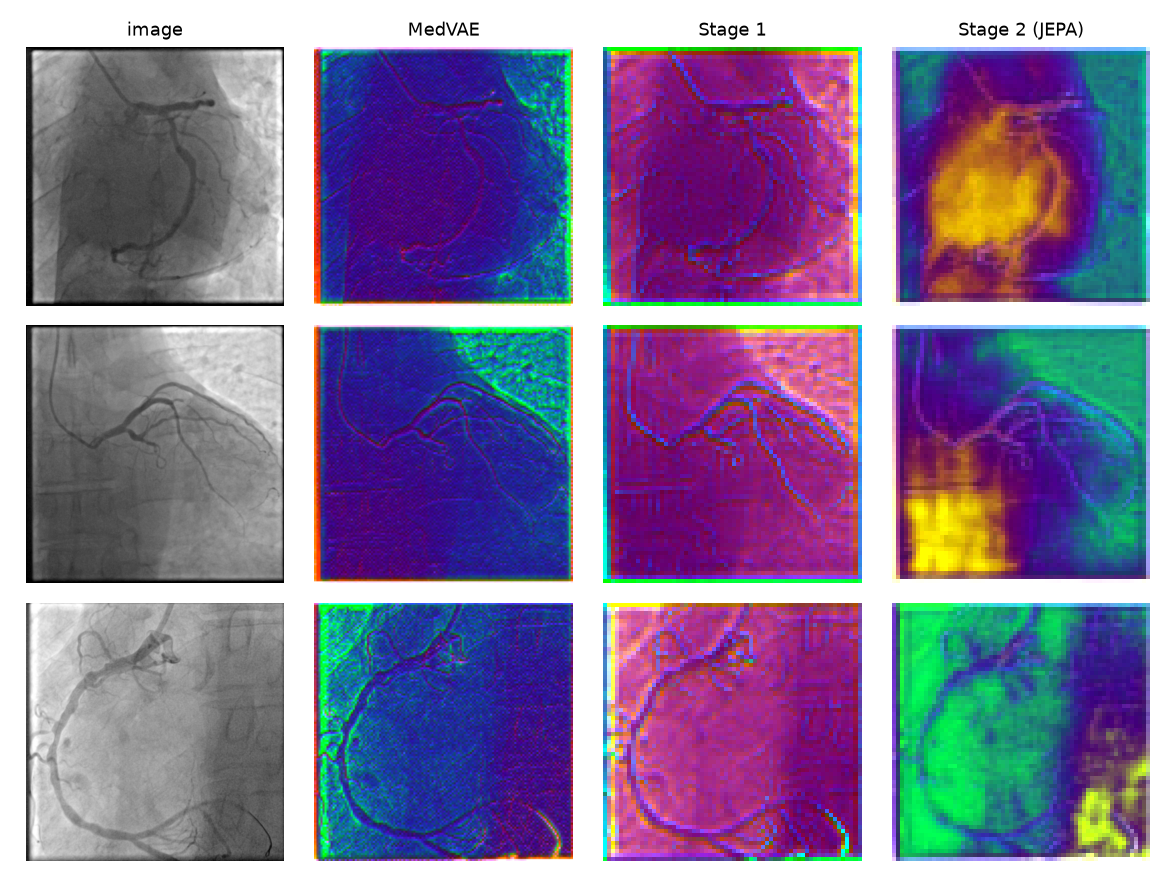
\includegraphics[height=0.78\textheight]{yanic/pca.png}

  \footnotesize Stage 2 features: large homogeneous regions, vessels barely visible.
\end{frame}

% ############################################################################
% PART 4 — THÉO
% Integration of MedVAE for multi-class segmentation
% Figures in figures/theo/
% ############################################################################
\section{Integration for multi-class segmentation}

\begin{frame}{Context and problem statement}
\begin{columns}[T]
\begin{column}{0.56\textwidth}
\textbf{Task.} Fine segmentation of coronary arteries on ARCADE:
\begin{itemize}
  \item 26 classes (the background and 25 segments)
  \item thin, tubular, low-contrast structures
  \item extreme imbalance ($\approx 95\,\%$ background)
\end{itemize}
\vspace{0.6em}
\textbf{Tool.} MedVAE, a pre-trained medical variational autoencoder: $\times 16$ compression in area ($512^2 \to 128^2 \times 1$), but \alert{lossy}.
\end{column}
\begin{column}{0.44\textwidth}
\begin{block}{Two questions}
\begin{enumerate}
  \item Does the compression preserve enough anatomical information for segmentation?
  \item Where to integrate it: \textbf{latent} space or \textbf{pixel} space?
\end{enumerate}
\end{block}
\end{column}
\end{columns}
\end{frame}

\begin{frame}{Method: five conditions}
\begin{columns}[c]
\begin{column}{0.36\textwidth}
\footnotesize
\begin{itemize}\setlength\itemsep{0.1em}
  \item \textbf{A} — full-resolution U-Net (reference)
  \item \textbf{A*} — U-Net from A on reconstructed images, \alert{without retraining} (control)
  \item \textbf{B} — U-Net head at the latent resolution, frozen MedVAE encoder
  \item \textbf{C} — like B, MedVAE fine-tuned on ARCADE
  \item \textbf{D} — U-Net retrained on reconstructed images
\end{itemize}
\vspace{0.3em}
\scriptsize 3 seeds per condition; artery Dice (background excluded) on the 300 test images.
\end{column}
\begin{column}{0.64\textwidth}
\centering
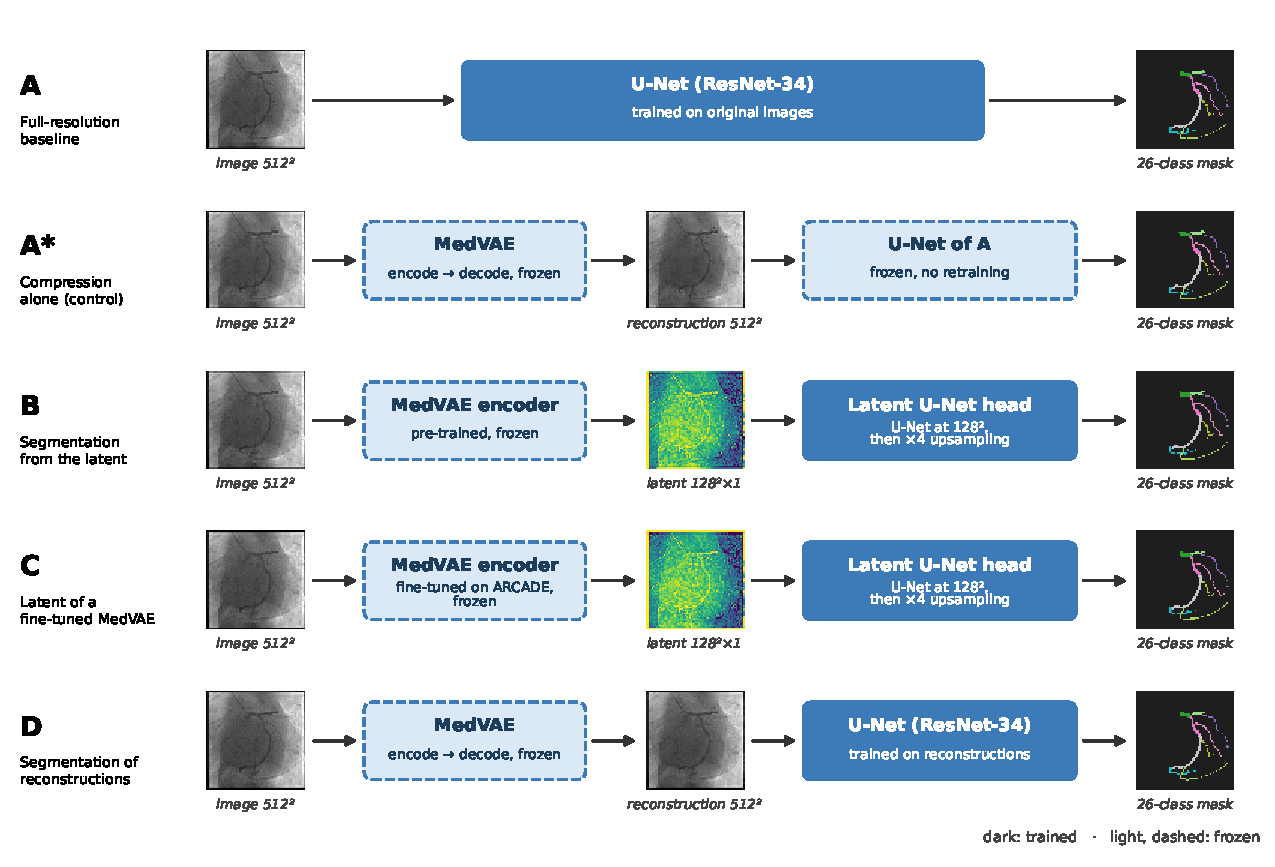
\includegraphics[width=\linewidth]{theo/conditions.pdf}
\end{column}
\end{columns}
\end{frame}

\begin{frame}{Result 1: segmentation from the latent works}
\begin{columns}[T]
\begin{column}{0.48\textwidth}
\small
\begin{itemize}
  \item B: \textbf{0.393}, C: \textbf{0.403} artery Dice, i.e.\ \textbf{91--94\,\%} of A (0.430), from a $16\times$ smaller input
  \item \alert{Earlier ``the latent fails'' (Dice 0.04)} was a training issue:
    \begin{itemize}\footnotesize
      \item head learning rate $5\times10^{-5}$, too low $\rightarrow 10^{-3}$
      \item no convolution at the latent resolution $\rightarrow$ small U-Net head
    \end{itemize}
  \item Fine-tuning MedVAE (C) helps slightly: C $\geq$ B on all seeds (+0.010)
\end{itemize}
\end{column}
\begin{column}{0.52\textwidth}
\centering
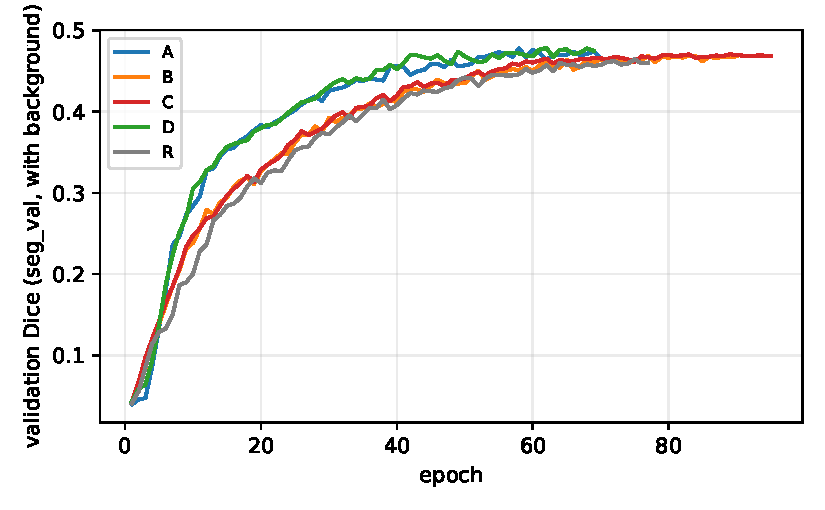
\includegraphics[width=\linewidth]{theo/seg_curves.pdf}

\footnotesize Validation Dice, mean over 3 seeds
\end{column}
\end{columns}
\end{frame}

\begin{frame}{Result 2: pixel space preserves, adaptation adds nothing}
\begin{columns}[T]
\begin{column}{0.42\textwidth}
\centering
\footnotesize
\begin{tabular}{lcc}
\toprule
Cond. & Artery Dice & Artery IoU \\
\midrule
A   & 0.430 $\pm$ 0.005 & 0.308 \\
A*  & 0.425 & 0.303 \\
B   & 0.393 $\pm$ 0.008 & 0.277 \\
C   & 0.403 $\pm$ 0.002 & 0.285 \\
D   & 0.432 $\pm$ 0.004 & 0.311 \\
\bottomrule
\end{tabular}
\end{column}
\begin{column}{0.58\textwidth}
\small
\begin{itemize}
  \item \textbf{Compression alone costs little}: A* $\approx$ A ($-0.006$)
  \item \textbf{D $\approx$ A} ($+0.003$, within seed variability)
  \item \alert{Earlier ``D gains on thin segments'' (+0.017)}: gone with 3 seeds and the corrected augmentation
\end{itemize}
\end{column}
\end{columns}
\vspace{0.2em}
\centering
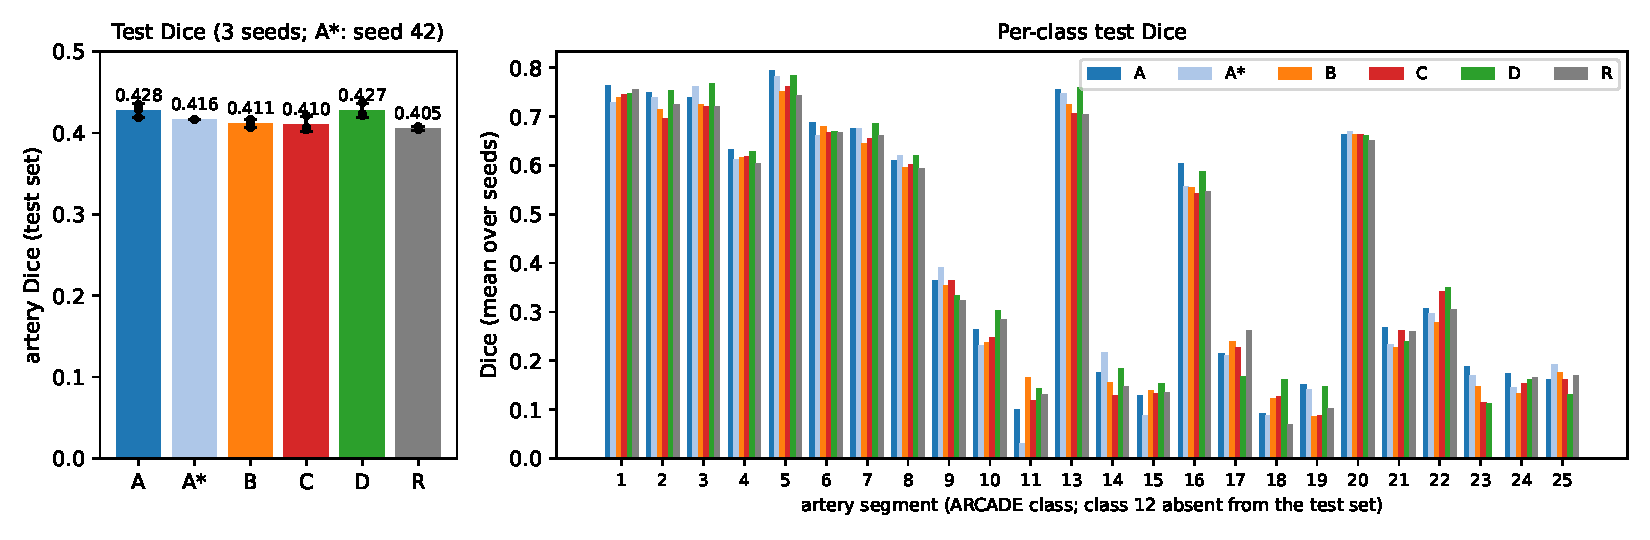
\includegraphics[width=0.84\textwidth]{theo/seg_results.pdf}
\end{frame}

\begin{frame}{Qualitative predictions}
\centering
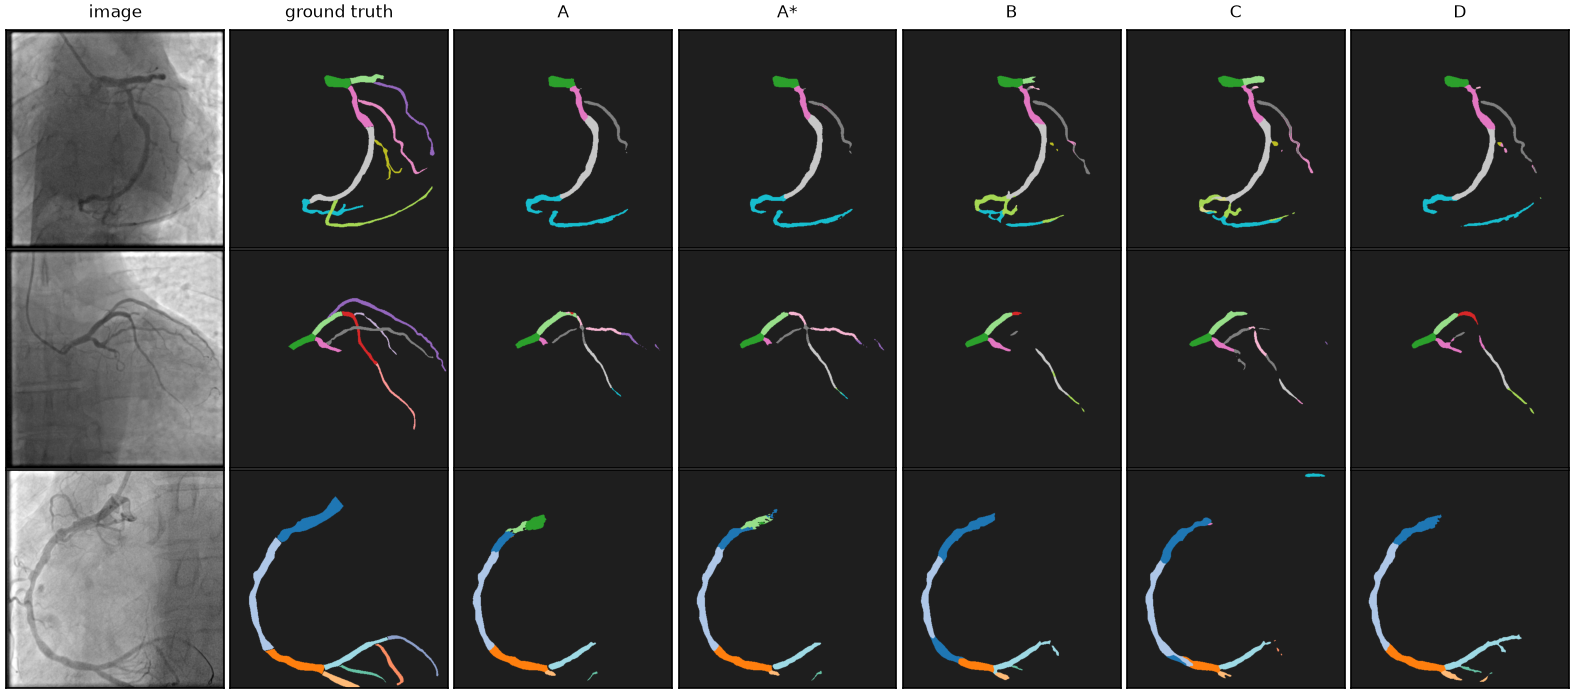
\includegraphics[width=0.9\textwidth]{theo/seg_predictions.png}

\footnotesize Seed-42 models on three test images: A, A* and D nearly identical; B and C follow the coronary tree from the $128\times128$ latent.
\end{frame}

% ############################################################################
% GENERAL CONCLUSION (from final.tex, Sec. Conclusion)
% ############################################################################
\begin{frame}{General conclusion}
  \footnotesize
  Across four complementary axes, we probed the behavior of MedVAE,
  a generic medical compressor, on the demanding domain of coronary angiography:
  \begin{itemize}
    \item \textbf{Robustness}: genuinely removes Poisson noise, restores neither JPEG
      nor blur --- and the denoising does \emph{not} make segmentation more robust.
    \item \textbf{FiLM}: fine-tuning on ARCADE gains 7 dB; conditioning on a quality
      score adds nothing, the score being a function of the image itself.
    \item \textbf{JEPA}: with a frozen decoder, degrades reconstruction and vessel
      separability; no dimensional contraction.
    \item \textbf{Segmentation}: $\times 16$ compression keeps the anatomy, in pixel
      space (D $\approx$ A) \emph{and} in the latent (91--94\,\% of A's Dice).
  \end{itemize}
  \vspace{0.3em}
  \textbf{Takeaway.} A faithful compression, reusable in pixel space and largely in its latent;
  several first-version conclusions reversed once the protocol was fixed
  (right reference, same training, several seeds, trained layer).
\end{frame}

% ############################################################################
% PERSPECTIVES (from final.tex, Sec. Perspectives)
% ############################################################################
\begin{frame}{Perspectives}
  \begin{block}{Toward a \emph{foundation model} for radiation-based medical imaging}
  Unify the explored axes into a single training objective.
  \end{block}
  \begin{itemize}
    \item \textbf{Hybrid JEPA + reconstruction objective}: predict the masked
      latent patches while keeping the encoder anchored to a decodable space.
    \item \textbf{Physically grounded degradations}: quantum noise,
      contrast/brightness, multiplicative fields, anisotropic motion blur
      (cardiac/respiratory).
    \item \textbf{Conditioning (CVAE)} on DICOM metadata \emph{not} derived from the image
      (modality, dose, acquisition parameters) $\rightarrow$ disentangled
      content / acquisition-quality representations.
    \item \textbf{Downstream validation}: classification, detection,
      multi-modality segmentation (ARCADE as a demanding test bed).
  \end{itemize}
\end{frame}



\end{document}